\subsection{Interface}

Ein\textbf{ User Interface (UI)} in eingebetteten Systemen ermöglicht eine Interaktion zwischen Benutzer und Gerät.

Das \textbf{Interface} besteht aus \textbf{Encodern}, \textbf{Schiebepotentiometern}, einem \textbf{LCD-Display }und \textbf{Buttons}. Dessen Zusammenspiel ermöglicht dem Benutzer die nötige Kontrolle über den Sampler.


Im folgenden Kapitel wird Ihnen die Funktionalität, Implementierung, Ansteuerung, sowie das Zusammenspiel der Komponenten untereinander nähergebracht: 

\subsubsection{Encoder und Display}

\textbf{Grundfunktionalität:}


Der \textbf{Encoder} dient der Navigation im Benutzer-Menü des Samplers. Er ermöglicht die Auswahl von Samples und das Scrollen durch die Sample-Liste, die auf dem LCD-Display angezeigt wird. Diese Liste zeigt die Namen der Samples an, die zuvor durch die Fader-Einstellungen bestimmt wurden. Der Cursor an der Seite zeigt die Aktuelle Position des Cursors an. Der Sample gilt als ausgewählt wen dessen Name unter der Liste erscheint.

\textbf{Umsetzung der Funktionalität:}

Die Auswahl von Samples sowie das Inkrementieren und Dekrementieren des Cursors, welcher sich im Struct des Filemanager befindet werden durch Interrupts unterstützt. Wenn der Encoder bewegt oder gedrückt wird, sendet er Signale an die MCU, die Interrupts auslösen.

Die Auswertung dieser Signale erfolgt dann in der Callback  \mintinline{c}|HAL_GPIO_EXTI_Callback(uint16_t GPIO_Pin)|. 

\begin{figure}[H]
	\centering
	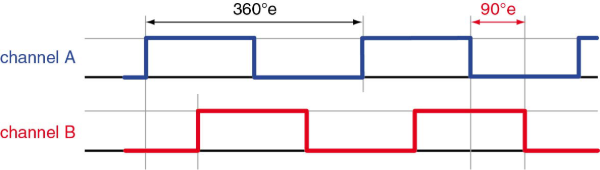
\includegraphics[width=0.8\textwidth]{images/08_durchfuehrung/interface/encoder.png}
	\caption{Phasenverschiebung A und B}
	\label{fig:phase_verschiebung}
\end{figure}

Wenn A und B beide High sind, wird die Cursor-Position welche in auf dem Display durch den Methodenaufruf \mintinline{c}|cursorUp(FileManager *fm)|
erhöht. Wenn A High und B Low ist, wird die Cursor-Position auf dem Display durch \mintinline{c}|cursorDown(FileManager *fm)| verringert. Wenn der Schalter gedrückt wird, wird die Datei durch \mintinline{c}|selectFile(FileManager *fm)| der Index des Files gespeichert und der Schalter wird mit Timer5 und dem Entprell-Flag entprellt, um mehrfach auslösungen zu verhindern.
 
 \inputminted[firstline=68, lastline=74]{c}{../../f401_display_encoder_fader_test/Core/Src/filemanager.c}
 
  \inputminted[firstline=84, lastline=90]{c}{../../f401_display_encoder_fader_test/Core/Src/filemanager.c}
  
Anhand des Index des Files kann der Names des Files ermittelt werden.

    \inputminted[firstline=159, lastline=161]{c}{../../f401_display_encoder_fader_test/Core/Src/filemanager.c}
  
 
\subsubsection{Schiebenpotentiometer, ADC und DMA}

\textbf{Schiebepotentiometer} erfassen analoge Spannungen, die vom \textbf{Analog-Digital-Wandler (ADC)} in digitale Werte umgewandelt werden. Der \textbf{Direct Memory Access (DMA)-Controller} übernimmt anschließend die direkte Übertragung dieser digitalen Werte in den Speicher, konkret in  \mintinline{c}|adcBuffer[NUM_CHANNELS]|, wodurch die CPU entlastet wird.

\begin{figure}[H]
	\centering
	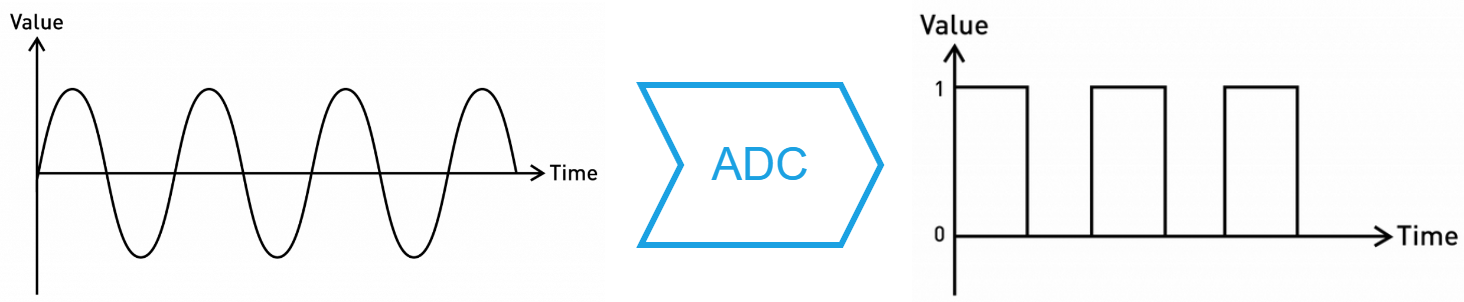
\includegraphics[width=1.0\textwidth]{images/08_durchfuehrung/interface/Conversion.drawio.png}
	\caption{ADC Conversion}
	\label{fig:conversion}
\end{figure}

\begin{figure}[H]
\centering
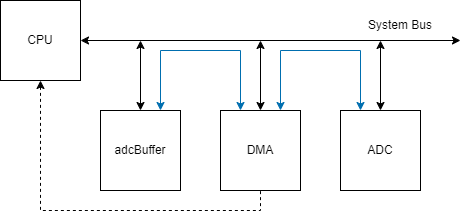
\includegraphics[width=1.0\textwidth]{images/08_durchfuehrung/interface/DMA_ADC_MEM.drawio.png}
\caption{DMA ADC FADER Bus System}
\label{fig:DMA ADC FADER}
\end{figure}

Die Auswertung und Verarbeitung der Signale erfolgt in der  \mintinline{c}| HAL_ADC_ConvCpltCallback(ADC_HandleTypeDef* hadc)|.

Zunächst werden die geglätteten Werte für alle Kanäle des ADC berechnet. Diese Glättung sorgt dafür, dass die Messwerte stabiler und weniger anfällig für zufällige Schwankungen sind. Anschließend werden die Durchschnittswerte ermittelt. Diese Durchschnittswerte dienen zwei Zwecken: Einerseits werden sie zur Anzeige auf dem Bildschirm verwendet, andererseits sind sie für Vergleichsoperationen innerhalb des Sortieralgorithmus von Bedeutung. Schließlich wird ein Zeichenarray initialisiert, das später auf dem Display angezeigt wird. Dieses Array enthält die aufbereiteten Daten, die dem Nutzer präsentiert werden.

 


